\documentclass[m3380-lec-main.tex]{subfiles}
\setcounter{chapter}{9}

%\DeclareMathOperator{\R}{\mathbb{R}}

\begin{document}


\chapter{Substitution Ciphers}

\section*{Goals}
\begin{enumerate}[1.~]\setlength{\itemsep}{0pt}
\item 
\end{enumerate}

\section*{Introduction}
A \emph{substitution cipher} in its simplest form is simply a permutation of the letters in an alphabet; more complicated substitution ciphers might map single characters to fixed-size blocks of characters.

\section{Simple substitution} Also called \emph{monoalphabetic substitution}, these are among the easiest encryptions to break. A simple substitution cipher employs a single permutation of the symbol set to encrypt the plaintext. The \emph{Caesar cipher} is one of the earliest known uses: in an alphabet of size $n$, the permutation for Julius Caesar's cipher was $\sigma(x) = (x+3)\mod n$. For Caesar's military dispatches, the permutation would have been
{\tiny\[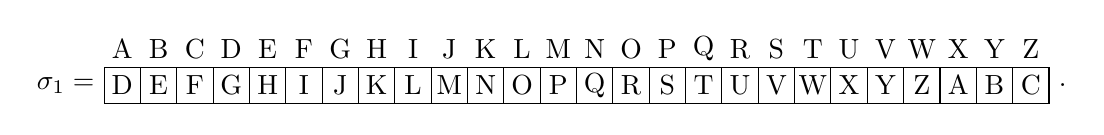
\begin{tikzpicture}[scale=12/26]
\draw (0,0.5) node [left] {$\sigma_1 =$} (0,0) grid (26,1) (26,0.5) node [right] {.};
\draw
    \foreach \x/\y in {A/0, B/1, C/2, D/3, E/4, F/5, G/6, H/7, I/8, J/9, K/10, L/11, M/12, N/13, O/14, P/15, Q/16, R/17, S/18, T/19, U/20, V/21, W/22, X/23, Y/24, Z/25}{ (\y+.5, 1.5) node {\x}}
    \foreach \x/\y in {D/0, E/1, F/2, G/3, H/4, I/5, J/6, K/7, L/8, M/9, N/10, O/11, P/12, Q/13, R/14, S/15, T/16, U/17, V/18, W/19, X/20, Y/21, Z/22, A/23, B/24, C/25}{ (\y+.5, 0.5) node {\x}};
\end{tikzpicture}
\]}
Since $26\equiv 1 \mod 3$, this permutation $\sigma_1$ would be written as a single $26$-cycle in disjoint cycle notation.

Generally speaking, we'll call an encryption of this type either a \emph{shift cipher} or a \emph{rotation cipher}; another frequently used rotation cipher is called ``ROT13," and is given by
{\tiny\[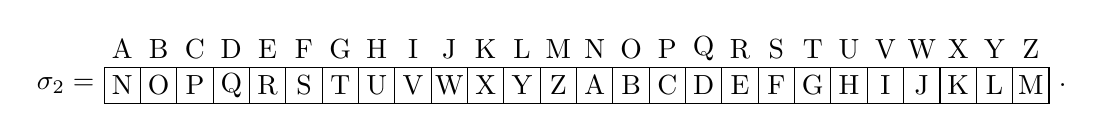
\begin{tikzpicture}[scale=12/26]
\draw (0,0.5) node [left] {$\sigma_2 =$} (0,0) grid (26,1) (26,0.5) node [right] {.};
\draw
    \foreach \x/\y in {A/0, B/1, C/2, D/3, E/4, F/5, G/6, H/7, I/8, J/9, K/10, L/11, M/12, N/13, O/14, P/15, Q/16, R/17, S/18, T/19, U/20, V/21, W/22, X/23, Y/24, Z/25}{ (\y+.5, 1.5) node {\x}}
    \foreach \x/\y in {N/0, O/1, P/2, Q/3, R/4, S/5, T/6, U/7, V/8, W/9, X/10, Y/11, Z/12, A/13, B/14, C/15, D/16, E/17, F/18, G/19, H/20, I/21, J/22, K/23, L/24, M/25}{ (\y+.5, 0.5) node {\x}};
\end{tikzpicture}
\]}
Since ROT13 is an involution\footnote{A permutation $\sigma$ is an involution if and only if $\sigma^2=(1)$.}, it is used as the canonical example of weak encryption; it was commonly used online in usenet newsgroups during the early 1980s to obscure text such as ``spoilers," punchlines to jokes, or obscene language.

\subsection{Polygraphic substitution} Another more secure technique is to permute groups of letters, effectively increasing the size of the alphabet. A digraph encryption would take pairs of adjacent letters (\emph{digraphs}) and permute them with another digraph. 

In the Playfair cipher\footnote{Developed in 1854 by Charles Wheatstone but advocated by Lord Playfair.} a $5\times 5$ grid of letters containing a keyword is memorized, along with four rules. The keyword is written into the grid, with duplicate letters removed, and the remaining letters follow. The letters $I$ and $J$ are written into the same position. For instance, if our key phrase is ``TALONS UP," the grid would be 
{\tiny\[

\begin{tikzpicture}[scale=1/3]
\draw \foreach \y/\x/\z in {4/0/T,  4/1/A,  4/2/L,  4/3/O,  4/4/N,  3/0/S,  3/1/U,  3/2/P,  3/3/B,  3/4/C,  2/0/D,  2/1/E,  2/2/F,  2/3/G,  2/4/H,  1/0/IJ,  1/1/K,  1/2/M,  1/3/Q,  1/4/R,  0/0/V,  0/1/W,  0/2/X,  0/3/Y,  0/4/Z}{
    (\x+.5,\y+.5) node {\z}
};
\end{tikzpicture}.
\]}
The rules are
\begin{enum}
\item If the paired letters are the same, insert an $X$ between them.
\item If the letters occur in the same row of the table, use the letters to their immediate right, wrapping around to the left side of the table if necessary.
\item If the letters occur in the same column of the table, use the letters immediately below them, wrapping around to the top of the table if necessary.
\item Otherwise, draw a rectangle around the pair of letters, and replace each with the unused corner from the same row.
\end{enum}
These rules are only difficult to formulate in writing, but in practice are easy to implement; the inventor claimed he could teach it to 3 out of 4 school boys in 15 minutes. To demonstrate the use of the cipher, we'll use our Playfair grid to encrypt the message, \verb|HIT THE BOOKKEEPER|. First, we break the plaintext into pairs, inserting $X$'s where necessary:
\[\texttt{HITTHEBOOKKEEPER}\mapsto \texttt{HI~T\underline{X}~TH~EB~O\underline{X}~OK~KE~EP~ER}\]

\noindent Next we draw the appropriate boxes, as demonstrated in \autoref{fig:playfair_exmp}.

\begin{figure}[hbt]
{\tiny\[
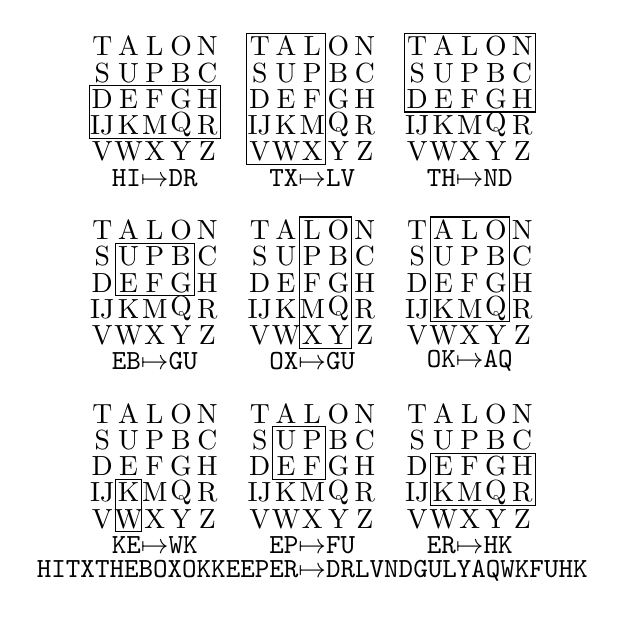
\begin{tikzpicture}[scale=1/3]
\draw \foreach \s in {0,6,12}{
    \foreach \t in {14, 7, 0}{
        \foreach \y/\x/\z in {4/0/T,  4/1/A,  4/2/L,  4/3/O,  4/4/N,  3/0/S,  3/1/U,  3/2/P,  3/3/B,  3/4/C,  2/0/D,  2/1/E,  2/2/F,  2/3/G,  2/4/H,  1/0/IJ,  1/1/K,  1/2/M,  1/3/Q,  1/4/R,  0/0/V,  0/1/W,  0/2/X,  0/3/Y,  0/4/Z}{
            (\s+\x+.5,\t+\y+.5) node {\z}
}}};
\draw
    (0,14 + 1) rectangle (5,14 + 3)
    (2.5,13.5) node {\texttt{HI}$\mapsto$\texttt{DR}}
    ( 6 + 0,14 + 0) rectangle ( 6 + 3,14 + 5)
    (8.5,13.5) node {\texttt{TX}$\mapsto$\texttt{LV}}
    (12 + 0,14 + 2) rectangle (12 + 5,14 + 5)
    (14.5,13.5) node {\texttt{TH}$\mapsto$\texttt{ND}}
    (1, 7 + 2) rectangle (4, 7 + 4)
    (2.5,6.5) node {\texttt{EB}$\mapsto$\texttt{GU}}
    ( 6 + 2, 7 + 0) rectangle ( 6 + 4, 7 + 5)
    (8.5,6.5) node {\texttt{OX}$\mapsto$\texttt{GU}}
    (12 + 1, 7 + 1) rectangle (12 + 4, 7 + 5)
    (14.5,6.5) node {\texttt{OK}$\mapsto$\texttt{AQ}}
    (1,0) rectangle (2,2)
    (2.5,-0.5) node {\texttt{KE}$\mapsto$\texttt{WK}}
    ( 6 + 1,2) rectangle ( 6 + 3,4)
    (8.5,-0.5) node {\texttt{EP}$\mapsto$\texttt{FU}}
    (12 + 1,1) rectangle (12 + 5,3)
    (14.5,-0.5) node {\texttt{ER}$\mapsto$\texttt{HK}};

\draw (8.5,-1.5) node {\texttt{HITXTHEBOXOKKEEPER$\mapsto$DRLVNDGULYAQWKFUHK}};
\end{tikzpicture}
\]}
\caption{\label{fig:playfair_exmp}Encoding characters using Playfair's cipher.}
\end{figure}

The resulting plaintext is \verb|DRLVN DGULY AQWKF UHK|, broken into 5-character blocks. To decrypt the message is to use the same Playfair grid and reverse rules 2, 3, and 4. Unfortunately, the use of this digraph substitution remains equivalent to a monoalphabetic substitution cipher, this time on an alphabet of $26\cdot 25 = 650$ symbols, since no double-letter digraphs are permuted. Since $\log_{10}(650!)\approx 1547.91$, this is a considerably large space of permutations to attack naively.

\section{Polyalphabetic substitution}
Polyalphabetic substitution still uses permutations to function, but \emph{the permutation changes between characters.} This presents sufficient difficulty to decryption that 

\newcommand{\vig}{Vigen\`{e}re~}

\subsection{The \vig Cipher}
The basis for the \vig cipher is the \emph{tabula recta}, a $26\times 26$ matrix of letters as shown in \autoref{fig:tabula_recta}.
\begin{figure}[hbt]
{\tiny\[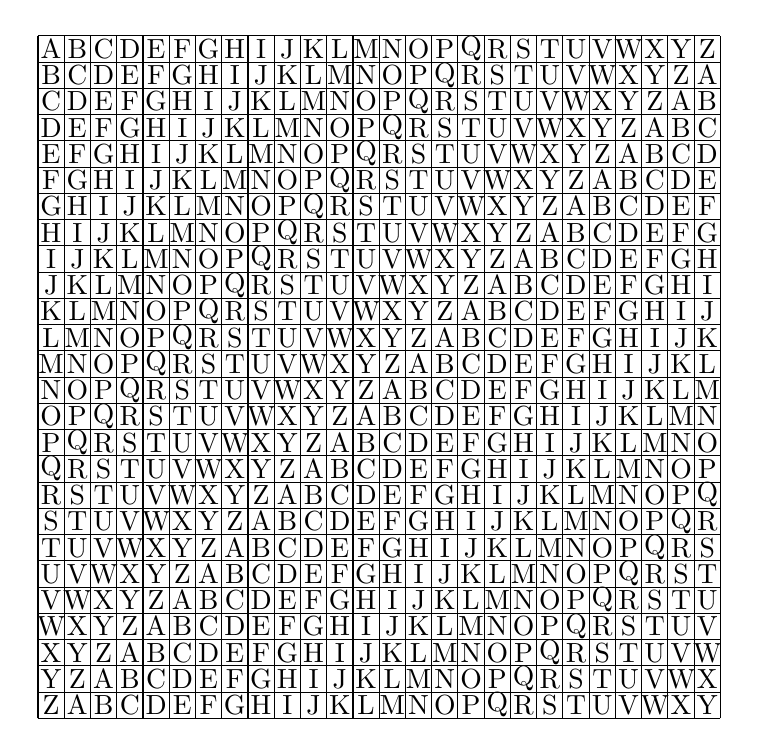
\begin{tikzpicture}[scale=1/3]
\draw[thin] (0,0) grid (26,26) \foreach \x/\y/\c in 
{0.5/25.5/A, 1.5/25.5/B, 2.5/25.5/C, 3.5/25.5/D, 4.5/25.5/E, 5.5/25.5/F, 6.5/25.5/G, 7.5/25.5/H, 8.5/25.5/I, 9.5/25.5/J, 10.5/25.5/K, 11.5/25.5/L, 12.5/25.5/M, 13.5/25.5/N, 14.5/25.5/O, 15.5/25.5/P, 16.5/25.5/Q, 17.5/25.5/R, 18.5/25.5/S, 19.5/25.5/T, 20.5/25.5/U, 21.5/25.5/V, 22.5/25.5/W, 23.5/25.5/X, 24.5/25.5/Y, 25.5/25.5/Z, 0.5/24.5/B, 1.5/24.5/C, 2.5/24.5/D, 3.5/24.5/E, 4.5/24.5/F, 5.5/24.5/G, 6.5/24.5/H, 7.5/24.5/I, 8.5/24.5/J, 9.5/24.5/K, 10.5/24.5/L, 11.5/24.5/M, 12.5/24.5/N, 13.5/24.5/O, 14.5/24.5/P, 15.5/24.5/Q, 16.5/24.5/R, 17.5/24.5/S, 18.5/24.5/T, 19.5/24.5/U, 20.5/24.5/V, 21.5/24.5/W, 22.5/24.5/X, 23.5/24.5/Y, 24.5/24.5/Z, 25.5/24.5/A, 0.5/23.5/C, 1.5/23.5/D, 2.5/23.5/E, 3.5/23.5/F, 4.5/23.5/G, 5.5/23.5/H, 6.5/23.5/I, 7.5/23.5/J, 8.5/23.5/K, 9.5/23.5/L, 10.5/23.5/M, 11.5/23.5/N, 12.5/23.5/O, 13.5/23.5/P, 14.5/23.5/Q, 15.5/23.5/R, 16.5/23.5/S, 17.5/23.5/T, 18.5/23.5/U, 19.5/23.5/V, 20.5/23.5/W, 21.5/23.5/X, 22.5/23.5/Y, 23.5/23.5/Z, 24.5/23.5/A, 25.5/23.5/B, 0.5/22.5/D, 1.5/22.5/E, 2.5/22.5/F, 3.5/22.5/G, 4.5/22.5/H, 5.5/22.5/I, 6.5/22.5/J, 7.5/22.5/K, 8.5/22.5/L, 9.5/22.5/M, 10.5/22.5/N, 11.5/22.5/O, 12.5/22.5/P, 13.5/22.5/Q, 14.5/22.5/R, 15.5/22.5/S, 16.5/22.5/T, 17.5/22.5/U, 18.5/22.5/V, 19.5/22.5/W, 20.5/22.5/X, 21.5/22.5/Y, 22.5/22.5/Z, 23.5/22.5/A, 24.5/22.5/B, 25.5/22.5/C, 0.5/21.5/E, 1.5/21.5/F, 2.5/21.5/G, 3.5/21.5/H, 4.5/21.5/I, 5.5/21.5/J, 6.5/21.5/K, 7.5/21.5/L, 8.5/21.5/M, 9.5/21.5/N, 10.5/21.5/O, 11.5/21.5/P, 12.5/21.5/Q, 13.5/21.5/R, 14.5/21.5/S, 15.5/21.5/T, 16.5/21.5/U, 17.5/21.5/V, 18.5/21.5/W, 19.5/21.5/X, 20.5/21.5/Y, 21.5/21.5/Z, 22.5/21.5/A, 23.5/21.5/B, 24.5/21.5/C, 25.5/21.5/D, 0.5/20.5/F, 1.5/20.5/G, 2.5/20.5/H, 3.5/20.5/I, 4.5/20.5/J, 5.5/20.5/K, 6.5/20.5/L, 7.5/20.5/M, 8.5/20.5/N, 9.5/20.5/O, 10.5/20.5/P, 11.5/20.5/Q, 12.5/20.5/R, 13.5/20.5/S, 14.5/20.5/T, 15.5/20.5/U, 16.5/20.5/V, 17.5/20.5/W, 18.5/20.5/X, 19.5/20.5/Y, 20.5/20.5/Z, 21.5/20.5/A, 22.5/20.5/B, 23.5/20.5/C, 24.5/20.5/D, 25.5/20.5/E, 0.5/19.5/G, 1.5/19.5/H, 2.5/19.5/I, 3.5/19.5/J, 4.5/19.5/K, 5.5/19.5/L, 6.5/19.5/M, 7.5/19.5/N, 8.5/19.5/O, 9.5/19.5/P, 10.5/19.5/Q, 11.5/19.5/R, 12.5/19.5/S, 13.5/19.5/T, 14.5/19.5/U, 15.5/19.5/V, 16.5/19.5/W, 17.5/19.5/X, 18.5/19.5/Y, 19.5/19.5/Z, 20.5/19.5/A, 21.5/19.5/B, 22.5/19.5/C, 23.5/19.5/D, 24.5/19.5/E, 25.5/19.5/F, 0.5/18.5/H, 1.5/18.5/I, 2.5/18.5/J, 3.5/18.5/K, 4.5/18.5/L, 5.5/18.5/M, 6.5/18.5/N, 7.5/18.5/O, 8.5/18.5/P, 9.5/18.5/Q, 10.5/18.5/R, 11.5/18.5/S, 12.5/18.5/T, 13.5/18.5/U, 14.5/18.5/V, 15.5/18.5/W, 16.5/18.5/X, 17.5/18.5/Y, 18.5/18.5/Z, 19.5/18.5/A, 20.5/18.5/B, 21.5/18.5/C, 22.5/18.5/D, 23.5/18.5/E, 24.5/18.5/F, 25.5/18.5/G, 0.5/17.5/I, 1.5/17.5/J, 2.5/17.5/K, 3.5/17.5/L, 4.5/17.5/M, 5.5/17.5/N, 6.5/17.5/O, 7.5/17.5/P, 8.5/17.5/Q, 9.5/17.5/R, 10.5/17.5/S, 11.5/17.5/T, 12.5/17.5/U, 13.5/17.5/V, 14.5/17.5/W, 15.5/17.5/X, 16.5/17.5/Y, 17.5/17.5/Z, 18.5/17.5/A, 19.5/17.5/B, 20.5/17.5/C, 21.5/17.5/D, 22.5/17.5/E, 23.5/17.5/F, 24.5/17.5/G, 25.5/17.5/H, 0.5/16.5/J, 1.5/16.5/K, 2.5/16.5/L, 3.5/16.5/M, 4.5/16.5/N, 5.5/16.5/O, 6.5/16.5/P, 7.5/16.5/Q, 8.5/16.5/R, 9.5/16.5/S, 10.5/16.5/T, 11.5/16.5/U, 12.5/16.5/V, 13.5/16.5/W, 14.5/16.5/X, 15.5/16.5/Y, 16.5/16.5/Z, 17.5/16.5/A, 18.5/16.5/B, 19.5/16.5/C, 20.5/16.5/D, 21.5/16.5/E, 22.5/16.5/F, 23.5/16.5/G, 24.5/16.5/H, 25.5/16.5/I, 0.5/15.5/K, 1.5/15.5/L, 2.5/15.5/M, 3.5/15.5/N, 4.5/15.5/O, 5.5/15.5/P, 6.5/15.5/Q, 7.5/15.5/R, 8.5/15.5/S, 9.5/15.5/T, 10.5/15.5/U, 11.5/15.5/V, 12.5/15.5/W, 13.5/15.5/X, 14.5/15.5/Y, 15.5/15.5/Z, 16.5/15.5/A, 17.5/15.5/B, 18.5/15.5/C, 19.5/15.5/D, 20.5/15.5/E, 21.5/15.5/F, 22.5/15.5/G, 23.5/15.5/H, 24.5/15.5/I, 25.5/15.5/J, 0.5/14.5/L, 1.5/14.5/M, 2.5/14.5/N, 3.5/14.5/O, 4.5/14.5/P, 5.5/14.5/Q, 6.5/14.5/R, 7.5/14.5/S, 8.5/14.5/T, 9.5/14.5/U, 10.5/14.5/V, 11.5/14.5/W, 12.5/14.5/X, 13.5/14.5/Y, 14.5/14.5/Z, 15.5/14.5/A, 16.5/14.5/B, 17.5/14.5/C, 18.5/14.5/D, 19.5/14.5/E, 20.5/14.5/F, 21.5/14.5/G, 22.5/14.5/H, 23.5/14.5/I, 24.5/14.5/J, 25.5/14.5/K, 0.5/13.5/M, 1.5/13.5/N, 2.5/13.5/O, 3.5/13.5/P, 4.5/13.5/Q, 5.5/13.5/R, 6.5/13.5/S, 7.5/13.5/T, 8.5/13.5/U, 9.5/13.5/V, 10.5/13.5/W, 11.5/13.5/X, 12.5/13.5/Y, 13.5/13.5/Z, 14.5/13.5/A, 15.5/13.5/B, 16.5/13.5/C, 17.5/13.5/D, 18.5/13.5/E, 19.5/13.5/F, 20.5/13.5/G, 21.5/13.5/H, 22.5/13.5/I, 23.5/13.5/J, 24.5/13.5/K, 25.5/13.5/L, 0.5/12.5/N, 1.5/12.5/O, 2.5/12.5/P, 3.5/12.5/Q, 4.5/12.5/R, 5.5/12.5/S, 6.5/12.5/T, 7.5/12.5/U, 8.5/12.5/V, 9.5/12.5/W, 10.5/12.5/X, 11.5/12.5/Y, 12.5/12.5/Z, 13.5/12.5/A, 14.5/12.5/B, 15.5/12.5/C, 16.5/12.5/D, 17.5/12.5/E, 18.5/12.5/F, 19.5/12.5/G, 20.5/12.5/H, 21.5/12.5/I, 22.5/12.5/J, 23.5/12.5/K, 24.5/12.5/L, 25.5/12.5/M, 0.5/11.5/O, 1.5/11.5/P, 2.5/11.5/Q, 3.5/11.5/R, 4.5/11.5/S, 5.5/11.5/T, 6.5/11.5/U, 7.5/11.5/V, 8.5/11.5/W, 9.5/11.5/X, 10.5/11.5/Y, 11.5/11.5/Z, 12.5/11.5/A, 13.5/11.5/B, 14.5/11.5/C, 15.5/11.5/D, 16.5/11.5/E, 17.5/11.5/F, 18.5/11.5/G, 19.5/11.5/H, 20.5/11.5/I, 21.5/11.5/J, 22.5/11.5/K, 23.5/11.5/L, 24.5/11.5/M, 25.5/11.5/N, 0.5/10.5/P, 1.5/10.5/Q, 2.5/10.5/R, 3.5/10.5/S, 4.5/10.5/T, 5.5/10.5/U, 6.5/10.5/V, 7.5/10.5/W, 8.5/10.5/X, 9.5/10.5/Y, 10.5/10.5/Z, 11.5/10.5/A, 12.5/10.5/B, 13.5/10.5/C, 14.5/10.5/D, 15.5/10.5/E, 16.5/10.5/F, 17.5/10.5/G, 18.5/10.5/H, 19.5/10.5/I, 20.5/10.5/J, 21.5/10.5/K, 22.5/10.5/L, 23.5/10.5/M, 24.5/10.5/N, 25.5/10.5/O, 0.5/9.5/Q, 1.5/9.5/R, 2.5/9.5/S, 3.5/9.5/T, 4.5/9.5/U, 5.5/9.5/V, 6.5/9.5/W, 7.5/9.5/X, 8.5/9.5/Y, 9.5/9.5/Z, 10.5/9.5/A, 11.5/9.5/B, 12.5/9.5/C, 13.5/9.5/D, 14.5/9.5/E, 15.5/9.5/F, 16.5/9.5/G, 17.5/9.5/H, 18.5/9.5/I, 19.5/9.5/J, 20.5/9.5/K, 21.5/9.5/L, 22.5/9.5/M, 23.5/9.5/N, 24.5/9.5/O, 25.5/9.5/P, 0.5/8.5/R, 1.5/8.5/S, 2.5/8.5/T, 3.5/8.5/U, 4.5/8.5/V, 5.5/8.5/W, 6.5/8.5/X, 7.5/8.5/Y, 8.5/8.5/Z, 9.5/8.5/A, 10.5/8.5/B, 11.5/8.5/C, 12.5/8.5/D, 13.5/8.5/E, 14.5/8.5/F, 15.5/8.5/G, 16.5/8.5/H, 17.5/8.5/I, 18.5/8.5/J, 19.5/8.5/K, 20.5/8.5/L, 21.5/8.5/M, 22.5/8.5/N, 23.5/8.5/O, 24.5/8.5/P, 25.5/8.5/Q, 0.5/7.5/S, 1.5/7.5/T, 2.5/7.5/U, 3.5/7.5/V, 4.5/7.5/W, 5.5/7.5/X, 6.5/7.5/Y, 7.5/7.5/Z, 8.5/7.5/A, 9.5/7.5/B, 10.5/7.5/C, 11.5/7.5/D, 12.5/7.5/E, 13.5/7.5/F, 14.5/7.5/G, 15.5/7.5/H, 16.5/7.5/I, 17.5/7.5/J, 18.5/7.5/K, 19.5/7.5/L, 20.5/7.5/M, 21.5/7.5/N, 22.5/7.5/O, 23.5/7.5/P, 24.5/7.5/Q, 25.5/7.5/R, 0.5/6.5/T, 1.5/6.5/U, 2.5/6.5/V, 3.5/6.5/W, 4.5/6.5/X, 5.5/6.5/Y, 6.5/6.5/Z, 7.5/6.5/A, 8.5/6.5/B, 9.5/6.5/C, 10.5/6.5/D, 11.5/6.5/E, 12.5/6.5/F, 13.5/6.5/G, 14.5/6.5/H, 15.5/6.5/I, 16.5/6.5/J, 17.5/6.5/K, 18.5/6.5/L, 19.5/6.5/M, 20.5/6.5/N, 21.5/6.5/O, 22.5/6.5/P, 23.5/6.5/Q, 24.5/6.5/R, 25.5/6.5/S, 0.5/5.5/U, 1.5/5.5/V, 2.5/5.5/W, 3.5/5.5/X, 4.5/5.5/Y, 5.5/5.5/Z, 6.5/5.5/A, 7.5/5.5/B, 8.5/5.5/C, 9.5/5.5/D, 10.5/5.5/E, 11.5/5.5/F, 12.5/5.5/G, 13.5/5.5/H, 14.5/5.5/I, 15.5/5.5/J, 16.5/5.5/K, 17.5/5.5/L, 18.5/5.5/M, 19.5/5.5/N, 20.5/5.5/O, 21.5/5.5/P, 22.5/5.5/Q, 23.5/5.5/R, 24.5/5.5/S, 25.5/5.5/T, 0.5/4.5/V, 1.5/4.5/W, 2.5/4.5/X, 3.5/4.5/Y, 4.5/4.5/Z, 5.5/4.5/A, 6.5/4.5/B, 7.5/4.5/C, 8.5/4.5/D, 9.5/4.5/E, 10.5/4.5/F, 11.5/4.5/G, 12.5/4.5/H, 13.5/4.5/I, 14.5/4.5/J, 15.5/4.5/K, 16.5/4.5/L, 17.5/4.5/M, 18.5/4.5/N, 19.5/4.5/O, 20.5/4.5/P, 21.5/4.5/Q, 22.5/4.5/R, 23.5/4.5/S, 24.5/4.5/T, 25.5/4.5/U, 0.5/3.5/W, 1.5/3.5/X, 2.5/3.5/Y, 3.5/3.5/Z, 4.5/3.5/A, 5.5/3.5/B, 6.5/3.5/C, 7.5/3.5/D, 8.5/3.5/E, 9.5/3.5/F, 10.5/3.5/G, 11.5/3.5/H, 12.5/3.5/I, 13.5/3.5/J, 14.5/3.5/K, 15.5/3.5/L, 16.5/3.5/M, 17.5/3.5/N, 18.5/3.5/O, 19.5/3.5/P, 20.5/3.5/Q, 21.5/3.5/R, 22.5/3.5/S, 23.5/3.5/T, 24.5/3.5/U, 25.5/3.5/V, 0.5/2.5/X, 1.5/2.5/Y, 2.5/2.5/Z, 3.5/2.5/A, 4.5/2.5/B, 5.5/2.5/C, 6.5/2.5/D, 7.5/2.5/E, 8.5/2.5/F, 9.5/2.5/G, 10.5/2.5/H, 11.5/2.5/I, 12.5/2.5/J, 13.5/2.5/K, 14.5/2.5/L, 15.5/2.5/M, 16.5/2.5/N, 17.5/2.5/O, 18.5/2.5/P, 19.5/2.5/Q, 20.5/2.5/R, 21.5/2.5/S, 22.5/2.5/T, 23.5/2.5/U, 24.5/2.5/V, 25.5/2.5/W, 0.5/1.5/Y, 1.5/1.5/Z, 2.5/1.5/A, 3.5/1.5/B, 4.5/1.5/C, 5.5/1.5/D, 6.5/1.5/E, 7.5/1.5/F, 8.5/1.5/G, 9.5/1.5/H, 10.5/1.5/I, 11.5/1.5/J, 12.5/1.5/K, 13.5/1.5/L, 14.5/1.5/M, 15.5/1.5/N, 16.5/1.5/O, 17.5/1.5/P, 18.5/1.5/Q, 19.5/1.5/R, 20.5/1.5/S, 21.5/1.5/T, 22.5/1.5/U, 23.5/1.5/V, 24.5/1.5/W, 25.5/1.5/X, 0.5/0.5/Z, 1.5/0.5/A, 2.5/0.5/B, 3.5/0.5/C, 4.5/0.5/D, 5.5/0.5/E, 6.5/0.5/F, 7.5/0.5/G, 8.5/0.5/H, 9.5/0.5/I, 10.5/0.5/J, 11.5/0.5/K, 12.5/0.5/L, 13.5/0.5/M, 14.5/0.5/N, 15.5/0.5/O, 16.5/0.5/P, 17.5/0.5/Q, 18.5/0.5/R, 19.5/0.5/S, 20.5/0.5/T, 21.5/0.5/U, 22.5/0.5/V, 23.5/0.5/W, 24.5/0.5/X, 25.5/0.5/Y}{
(\x,\y) node {\c}
};
\end{tikzpicture}\]}
\caption{\label{fig:tabula_recta}The \emph{tabula recta} used in the \vig cipher and other polyalphabetic substitutions.}
\end{figure}
Rather than simply using one shift cipher, this tabula recta incorporates every shift cipher. The process for using it is as follows: 
\begin{enum}
\item Select a keyword or keyphrase.
\item Write the plain text in one line.
\item Write the keyphrase repeatedly beneath the plain text.
\item The letter of the keyphrase determines which row of the tabula recta to look at, and the corresponding letter of the plain text determines which column.
\end{enum}
For instance, if our key phrase is \[\verb|"THIS PARROT HAS CEASED TO BE"|\] and our plain text is \[\verb|"THATS ONE SMALL STEP FOR A MAN ONE GIANT LEAP FOR MANKIND"|,\] we would write (blocking the message into 5-character blocks for readability)
{\tiny\[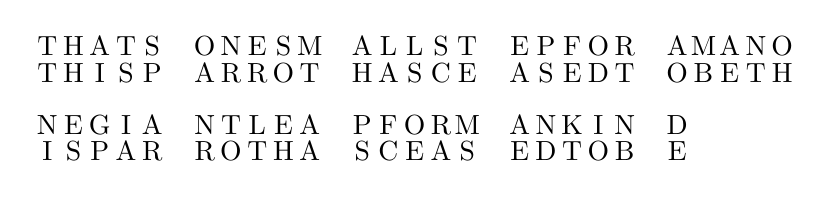
\begin{tikzpicture}[scale=1/3]
\draw \foreach \x/\y/\p/\k in {0/3/T/T, 1/3/H/H, 2/3/A/I, 3/3/T/S, 4/3/S/P, 6/3/O/A, 7/3/N/R, 8/3/E/R, 9/3/S/O, 10/3/M/T, 12/3/A/H, 13/3/L/A, 14/3/L/S, 15/3/S/C, 16/3/T/E, 18/3/E/A, 19/3/P/S, 20/3/F/E, 21/3/O/D, 22/3/R/T, 24/3/A/O, 25/3/M/B, 26/3/A/E, 27/3/N/T, 28/3/O/H, 0/0/N/I, 1/0/E/S, 2/0/G/P, 3/0/I/A, 4/0/A/R, 6/0/N/R, 7/0/T/O, 8/0/L/T, 9/0/E/H, 10/0/A/A, 12/0/P/S, 13/0/F/C, 14/0/O/E, 15/0/R/A, 16/0/M/S, 18/0/A/E, 19/0/N/D, 20/0/K/T, 21/0/I/O, 22/0/N/B, 24/0/D/E}{
(\x+.5,\y+.5) node {\k} (\x+.5,\y+1.5) node {\p}
};
\end{tikzpicture}.
\]}
We then proceed to use the tabula recta: since the first character of the key phrase is a \verb|T|, we look in the row beginning with \verb|T|; we then find the column beginning with \verb|T|, as \verb|T| is the first character of the message. The letter in the \verb|T|$^\text{th}$ row and \verb|T|$^\text{th}$ column is \verb|M|. Proceeding in this manner we obtain the cyphertext:
\[\verb|MOILH OEVGF HLDUX EHJRK ONEGV VWVIR EHELA HHSRE EQDWO H|.\]

\subsection{The Enigma Cipher} Perhaps the most famous modern polyalphabetic substitution cipher is Enigma, used by Nazi Germany during World War II to encrypt its military transmissions. The Enigma machines were not computers -- early versions were machines which used a series of rotors to encode messages between a keyboard and a lampboard, while later machines were modified to print messages directly onto a narrow paper strip.

Enigma machines had a varying number of permutation rotors at different stages of the war, as well as a ``plugboard". Each rotor was a plastic disc with 26 spring-loaded electrical contact pins on one side and 26 corresponding contact plates on the other side. Connecting pins on one side to plates on the other was a wiring which corresponds to a permutation of the 26 signals. Assuming a 3-rotor Enigma, the electrical path of a signal would pass from the key to the plugboard, to the entry wheel, then through the three rotors -- right, middle, then left. Finally, there was an element called a reflector, which acted as an \emph{involution}, and then the path went through the rotors again, but reversed -- left, right, middle. The electrical signal then would pass again through the plugboard and to the lamps. Both plugboard and reflector were reconfigurable.

Further, when a key was released, the rotation mechanism would engage. The right rotor would step, and upon reaching a notch in its mechanism would make the middle rotor step. This in turn could turn the left rotor in the same way. Of the eight rotors in use during World War II, rotors VI, VII, and VIII each had two such notches, providing an irregular stepping to break up the odometer-style pattern of rotor stepping. The result of this stepping mathematically is equivalent to shifting \emph{just the bottom row} of the two-line notation for that rotor's permutation by one position to the left. It is this stepping which makes Enigma polyalphabetic -- the permutation changes with each letter encrypted.

A further feature of the Enigma machine is that every setting of rotors and plugboard results in a \emph{derangement}. This feature was patented prior to World War II, when Enigma was sold commercially, and greatly aided Polish algebraist Marian Rejewski in his work to break the  encryption.

\begin{defn} A \emph{derangement} is a permutation with no fixed points.
\end{defn}

Coupling the use of derangements with the knowledge that the same machine had to encrypt and decrypt the message using the same settings, Rejewski and others were able to devise mathematical theory which allowed the Enigma to be broken. For instance, consider the permutations as follows:
\begin{align*}
P &= \text{plugboard} \\
R &= \text{right rotor} \\
M &= \text{middle rotor} \\
L &= \text{left rotor} \\
U &= \text{reflector}
\end{align*}
Then we know certain things from permutation theory and the design of the Enigma machine. First, we know that $P$ and $U$ are involutions: $P^2 = U^2 = (1)$. Further, we know that
\[ E = PRMLUL^{-1}M^{-1}R^{-1}P^{-1} \] is a derangement, as is
\[ E_{i,j,k} = P(\rho^i R\rho^{-i})(\rho^j M\rho^{-j})(\rho^k L\rho^{-k})U(\rho^k L^{-1}\rho^{-k})(\rho^j M^{-1}\rho^{-j})(\rho^i R^{-1}\rho^{-i})P^{-1},\]
the permutation after stepping each rotor the specified number of times. With three rotors installed out of a set of five, 26 different initial rotor settings for each installed rotor, a configurable reflector, and a plugboard with up to ten pairs of letters transposed, the military version of Enigma could be configured to a staggering number of initial settings
initial settings. Each of these can be considered the ``key phrase."

The use of the initial rotor setting was only intended to be used for transmission of the individual message key: the correct code book setting for the rotors would be set, then some ``randomly selected" three-letter \emph{message key} would be selected. This would be sent through the Enigma twice consecutively. Once this was completed, the rotors were set to the positions of the message key and encoding of the actual message would commence. The message key could be read off the initial rotor settings in normal left-to-right order.

\begin{exmp} The actual rotor wirings -- and the permutations they produce -- can be found by a quick web search. Even more interesting  is that key pages from the Luftwaffe survived the war and can be found! The key settings for day 30 of Luftwaffe Machine Key no. 649, reproduced from Wikipedia, specifies rotors I, V, and III, with ring settings 14, 09 24. The reflector setting is \texttt{KM AX PZ GO DI CN BR PV LT EQ HS UW}, and the plugboard is to be set to \texttt{SZ GT DV KU FO MY EW JN IX LQ}. Further, we'll use the first of the ground settigns, \verb|wny|. Suppose I choose my message key to be \verb|qzv|. I begin by encoding \verb|qzv| twice under ground setting \verb|wny|, given the correct initialization. 

\begin{figure}[hbt]{\tiny
\[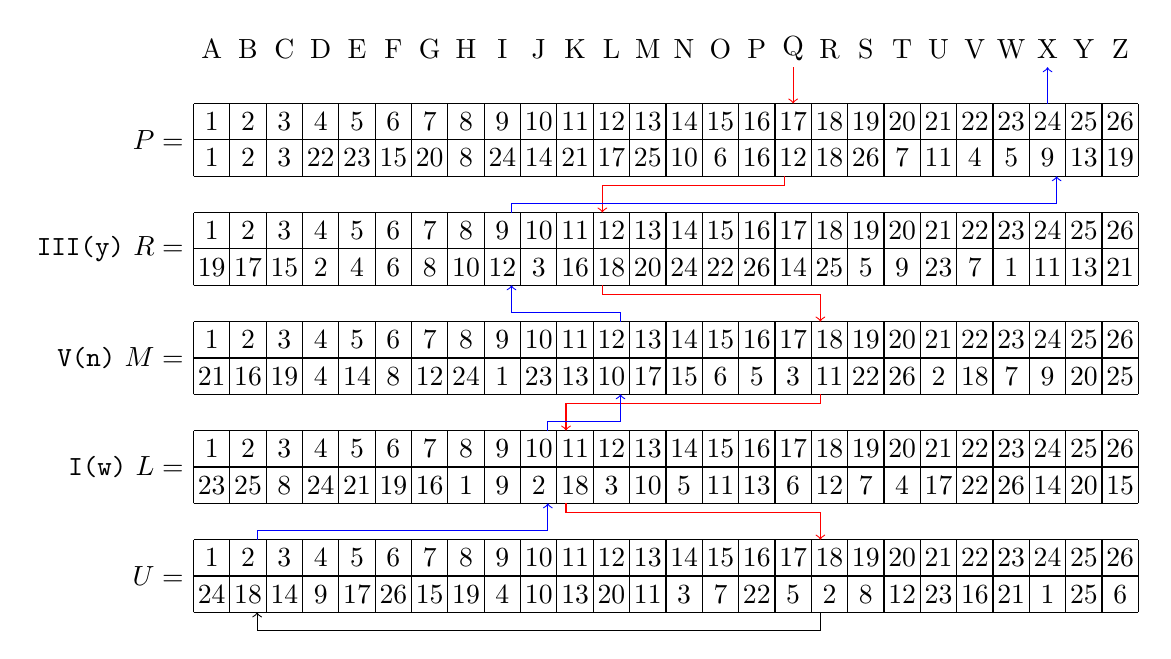
\begin{tikzpicture}[scale = 12/26]
\draw \foreach \x/\c in {1/A, 2/B, 3/C, 4/D, 5/E, 6/F, 7/G, 8/H, 9/I, 10/J, 11/K, 12/L, 13/M, 14/N, 15/O, 16/P, 17/Q, 18/R, 19/S, 20/T, 21/U, 22/V, 23/W, 24/X, 25/Y, 26/Z}{ (\x-0.5,0.5) node {\c}};
\draw (0,-2) node [left] {$P=$};
\draw (0, -5) node [left] {\texttt{III(y)}~$R=$};
\draw (0, -8) node [left] {\texttt{V(n)}~$M=$};
\draw (0,-11) node [left] {\texttt{I(w)}~$L=$};
\draw (0,-14) node [left] {$U=$};
%
\draw (0,-3) grid (26,-1)
	\foreach \x in {1,...,26}{(\x-0.5,-1.5) node {\x}}
	\foreach \x/\c in {1/1, 2/2, 3/3, 4/22, 5/23, 6/15, 7/20, 8/8, 9/24, 10/14, 11/21, 12/17, 13/25, 14/10, 15/6, 16/16, 17/12, 18/18, 19/26, 20/7, 21/11, 22/4, 23/5, 24/9, 25/13, 26/19}{(\x-0.5,-2.5) node {\c}};
\draw (0,-6) grid (26,-4)
	\foreach \x in {1,...,26}{(\x-0.5,-4.5) node {\x}}
	\foreach \x/\c in {1/19, 2/17, 3/15, 4/2, 5/4, 6/6, 7/8, 8/10, 9/12, 10/3, 11/16, 12/18, 13/20, 14/24, 15/22, 16/26, 17/14, 18/25, 19/5, 20/9, 21/23, 22/7, 23/1, 24/11, 25/13, 26/21}{(\x-0.5,-5.5) node {\c}};
\draw (0,-9) grid (26,-7)
	\foreach \x in {1,...,26}{(\x-0.5,-7.5) node {\x}}
	\foreach \x/\c in {1/21, 2/16, 3/19, 4/4, 5/14, 6/8, 7/12, 8/24, 9/1, 10/23, 11/13, 12/10, 13/17, 14/15, 15/6, 16/5, 17/3, 18/11, 19/22, 20/26, 21/2, 22/18, 23/7, 24/9, 25/20, 26/25}{(\x-0.5,-8.5) node {\c}};
\draw (0,-12) grid (26,-10)
	\foreach \x in {1,...,26}{(\x-0.5,-10.5) node {\x}}
	\foreach \x/\c in {1/23, 2/25, 3/8, 4/24, 5/21, 6/19, 7/16, 8/1, 9/9, 10/2, 11/18, 12/3, 13/10, 14/5, 15/11, 16/13, 17/6, 18/12, 19/7, 20/4, 21/17, 22/22, 23/26, 24/14, 25/20, 26/15}{(\x-0.5,-11.5) node {\c}};
\draw (0,-15) grid (26,-13)
	\foreach \x in {1,...,26}{(\x-0.5,-13.5) node {\x}}
	\foreach \x/\c in {1/24, 2/18, 3/14, 4/9, 5/17, 6/26, 7/15, 8/19, 9/4, 10/10, 11/13, 12/20, 13/11, 14/3, 15/7, 16/22, 17/5, 18/2, 19/8, 20/12, 21/23, 22/16, 23/21, 24/1, 25/25, 26/6}{(\x-0.5,-14.5) node {\c}};
%
\draw [->, draw=red] (16.5,0) -- (16.5,-1);
\draw [->, draw=red] (16.25,-3) -- (16.25,-3.25) -- (11.25,-3.25) -- (11.25,-4);
\draw [->, draw=red] (11.25,-6) -- (11.25,-6.25) -- (17.25,-6.25) -- (17.25,-7);
\draw [->, draw=red] (17.25,-9) -- (17.25,-9.25) -- (10.25,-9.25) -- (10.25,-10);
\draw [->, draw=red] (10.25,-12) -- (10.25,-12.25) -- (17.25,-12.25) -- (17.25,-13);
\draw [->, draw=black] (17.25,-15) -- (17.25,-15.5) -- (1.75,-15.5) -- (1.75,-15);
\draw [->, draw=blue] (1.75,-13) -- (1.75,-12.75) -- (9.75,-12.75) -- (9.75,-12);
\draw [->, draw=blue] (9.75,-10) -- (9.75,-9.75) -- (11.75, -9.75) -- (11.75,-9);
\draw [->, draw=blue] (11.75,-7) -- (11.75, -6.75) -- (8.75,-6.75) -- (8.75,-6);
\draw [->, draw=blue] (8.75,-4) -- (8.75,-3.75) -- (23.75,-3.75) -- (23.75,-3);
\draw [->, draw=blue] (23.5,-1) -- (23.5,0);
\end{tikzpicture}
\]}
\caption{\label{fig:enigma_1} The beginning of sending a message indicator using Enigma maps \texttt{Q} to \texttt{P}.}
\end{figure}
The electrical pathway traced through the plugboard, rotors, and reflector is demonstrated in \autoref{fig:enigma_1}. After \verb|Q| is pressed, \verb|X| lights up. When \verb|Q| is released, we see that the right-most rotor is not in position to step its neighbor, so only that rotor will step. The next pathway is demonstrated in \autoref{fig:enigma_2}.

\begin{figure}[hbt]{\tiny
\[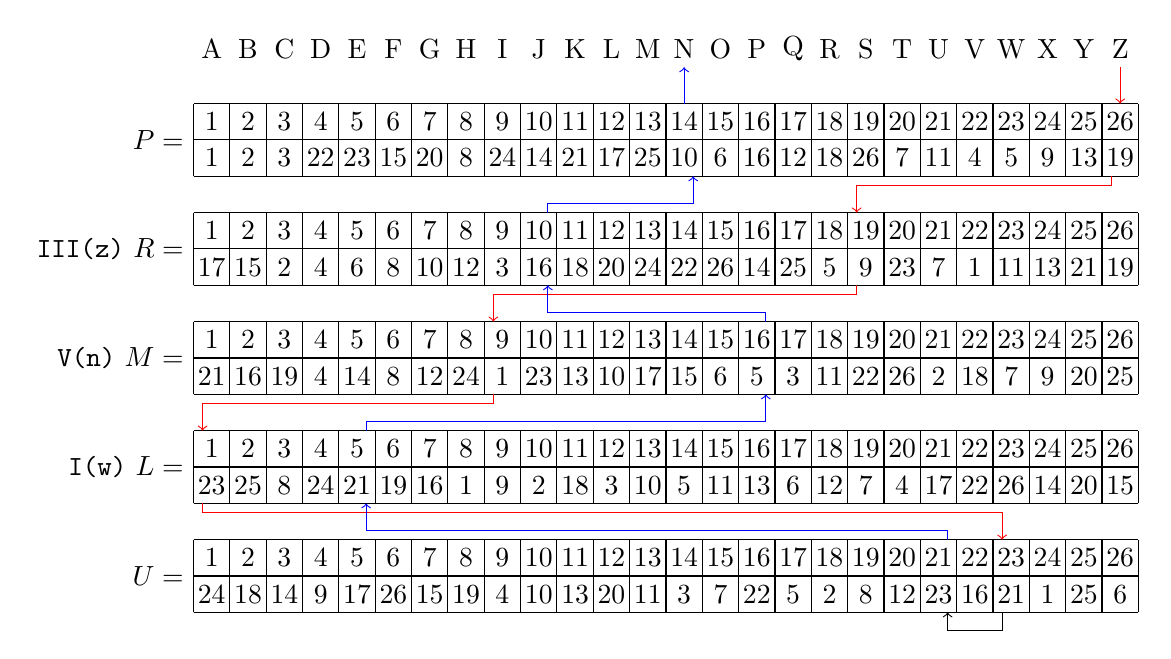
\begin{tikzpicture}[scale=12/26]
\draw \foreach \x/\c in {1/A, 2/B, 3/C, 4/D, 5/E, 6/F, 7/G, 8/H, 9/I, 10/J, 11/K, 12/L, 13/M, 14/N, 15/O, 16/P, 17/Q, 18/R, 19/S, 20/T, 21/U, 22/V, 23/W, 24/X, 25/Y, 26/Z}{ (\x-0.5,0.5) node {\c}};
\draw (0,-2) node [left] {$P=$};
\draw (0, -5) node [left] {\texttt{III(z)}~$R=$};
\draw (0, -8) node [left] {\texttt{V(n)}~$M=$};
\draw (0,-11) node [left] {\texttt{I(w)}~$L=$};
\draw (0,-14) node [left] {$U=$};
%
\draw (0,-3) grid (26,-1)
	\foreach \x in {1,...,26}{(\x-0.5,-1.5) node {\x}}
	\foreach \x/\c in {1/1, 2/2, 3/3, 4/22, 5/23, 6/15, 7/20, 8/8, 9/24, 10/14, 11/21, 12/17, 13/25, 14/10, 15/6, 16/16, 17/12, 18/18, 19/26, 20/7, 21/11, 22/4, 23/5, 24/9, 25/13, 26/19}{(\x-0.5,-2.5) node {\c}};
\draw (0,-6) grid (26,-4)
	\foreach \x in {1,...,26}{(\x-0.5,-4.5) node {\x}}
	\foreach \x/\c in {1/17, 2/15, 3/2, 4/4, 5/6, 6/8, 7/10, 8/12, 9/3, 10/16, 11/18, 12/20, 13/24, 14/22, 15/26, 16/14, 17/25, 18/5, 19/9, 20/23, 21/7, 22/1, 23/11, 24/13, 25/21, 26/19}{(\x-0.5,-5.5) node {\c}};
\draw (0,-9) grid (26,-7)
	\foreach \x in {1,...,26}{(\x-0.5,-7.5) node {\x}}
	\foreach \x/\c in {1/21, 2/16, 3/19, 4/4, 5/14, 6/8, 7/12, 8/24, 9/1, 10/23, 11/13, 12/10, 13/17, 14/15, 15/6, 16/5, 17/3, 18/11, 19/22, 20/26, 21/2, 22/18, 23/7, 24/9, 25/20, 26/25}{(\x-0.5,-8.5) node {\c}};
\draw (0,-12) grid (26,-10)
	\foreach \x in {1,...,26}{(\x-0.5,-10.5) node {\x}}
	\foreach \x/\c in {1/23, 2/25, 3/8, 4/24, 5/21, 6/19, 7/16, 8/1, 9/9, 10/2, 11/18, 12/3, 13/10, 14/5, 15/11, 16/13, 17/6, 18/12, 19/7, 20/4, 21/17, 22/22, 23/26, 24/14, 25/20, 26/15}{(\x-0.5,-11.5) node {\c}};
\draw (0,-15) grid (26,-13)
	\foreach \x in {1,...,26}{(\x-0.5,-13.5) node {\x}}
	\foreach \x/\c in {1/24, 2/18, 3/14, 4/9, 5/17, 6/26, 7/15, 8/19, 9/4, 10/10, 11/13, 12/20, 13/11, 14/3, 15/7, 16/22, 17/5, 18/2, 19/8, 20/12, 21/23, 22/16, 23/21, 24/1, 25/25, 26/6}{(\x-0.5,-14.5) node {\c}};
%
\draw [->, draw=red] (25.5,0) -- (25.5,-1);
\draw [->, draw=red] (25.25,-3) -- (25.25,-3.25) -- (18.25,-3.25) -- (18.25,-4);
\draw [->, draw=red] (18.25,-6) -- (18.25,-6.25) -- (8.25, -6.25) -- (8.25, -7);
\draw [->, draw=red] (8.25,-9) -- (8.25,-9.25) -- (0.25, -9.25) -- (0.25, -10);
\draw [->, draw=red] (0.25,-12) -- (0.25,-12.25) -- (22.25,-12.25) -- (22.25,-13);
\draw [->, draw=black] (22.25,-15) -- (22.25,-15.5) -- (20.75,-15.5) -- (20.75,-15);
\draw [->, draw=blue] (20.75,-13) -- (20.75,-12.75) -- (4.75,-12.75) -- (4.75,-12);
\draw [->, draw=blue] (4.75,-10) -- (4.75,-9.75) -- (15.75, -9.75) -- (15.75,-9);
\draw [->, draw=blue] (15.75,-7) -- (15.75, -6.75) -- (9.75,-6.75) -- (9.75,-6);
\draw [->, draw=blue] (9.75,-4) -- (9.75,-3.75) -- (13.75,-3.75) -- (13.75,-3);
\draw [->, draw=blue] (13.5,-1) -- (13.5,0);
\end{tikzpicture}\]}
\caption{\label{fig:enigma_2}The second character encoding of the same message indicator maps \texttt{Z} to \texttt{N}.}
\end{figure}

Further diagrams can be drawn, demonstrating the turning rotors as the message indicator \verb|QZVQZV| is encrypted to \verb|XNCYFT|. The rotors are then manually set to positions \verb|QZV| and the secret message begins being encrypted. If the full message you intercept is 
\begin{align*}
\texttt{XNCYF TSIXR VIVGQ MXVFO AHOLR YLZUN EEHDT GOAXT GRYVO}\\
\texttt{ALGPV OCBAK HTDVB VLFKD QPPKV UAYRZ ANYGY IHHFE GFJM~}
\end{align*}
can you decipher it, knowing my initial settings of the Enigma?
\end{exmp}

\end{document}


